\documentclass{article}
\usepackage{pdfpages}
\usepackage{xeCJK}
\usepackage{amsmath}
\usepackage{amssymb}
\usepackage{amsfonts}
\setCJKmainfont{Noto Serif CJK SC}
\usepackage[a4paper, total={170mm,257mm}, left=20mm, top=20mm]{geometry}
\usepackage{enumitem}
\usepackage{indentfirst}
\usepackage{graphicx}
\usepackage{graphics}
\usepackage{float}
\usepackage{algorithmicx}
\usepackage{hyperref}

\DeclareMathOperator*{\argmax}{arg\,max}
\DeclareMathOperator*{\argmin}{arg\,min}

% \usepackage[margin=0.3cm]{geometry}
\usepackage{hyperref}
\hypersetup{colorlinks=true,
    linkcolor=blue,
    filecolor=magenta,      
    urlcolor=cyan,
    pdftitle={SI140 project report: analysis and discussions},
}
\urlstyle{same}

\usepackage[
   backend=biber,
   style=alphabetic,
   sorting=ynt
]{biblatex}
\addbibresource{ref.bib}

\usepackage{fancyhdr}
\pagestyle{fancy}
\fancyhf{}
\lfoot{SI140 Final Project}
\cfoot{multi-armed bandit learning}
\rfoot{Page \thepage}
\renewcommand{\headrulewidth}{1pt}
\renewcommand{\footrulewidth}{1pt}
\setlength{\headsep}{10pt}

\newenvironment{newSec}[1]{
	\section{#1}
	\lhead{#1}
	\chead{}
	\rhead{}
}{ \newpage }
\newenvironment{newSubSec}[1]{
	\subsection{#1}
}{}

\newcommand{\ic}[2]{\centering \includegraphics[scale={#1}]{#2}}

\begin{document}
\title{
	{Performance Evaluation on Classical Algorithms for Multi-Armed Bandit}
		{SI140@2021Fall final project}
}
\author{Cheng Peng\thanks{\href{mailto:pengcheng2@shanghaitech.edu.cn}{pengcheng2@shanghaitech.edu.cn}\quad ID=2020533068}}
\maketitle
\tableofcontents
\newpage

\begin{newSec}{The Overall Performance Comparison}
	We made a bar chart\ref{fig:bc} based on the simulation,
	where the length of each bar is the gap\footnote{This is also called \textit{regret}, which is the goal to minimize.} between the oracle value and the average reward of the corresponding algorithm.\\
	Generally speaking, we have $\mathrm{TS}>\mathrm{UCB}>\mathrm{\epsilon\!-\!Greedy}$ in the sense of average reward, when the parameter is tuned.\par


	\begin{figure}[!htbp]
		\label{fig:bc}
		\ic{0.4}{pic/compare-bar.png}\\
		\ic{0.5}{pic/compare-label.png}\\
		\caption{Bar Chart: the performance of each algorithms}
	\end{figure}

	\vspace{4ex}

	To better understand the behavior of each algorithm, the knowledge used to make decision on each step is recorded. We store the estimated $\theta_j$s and organize them into {scatter plots}\ref{fig:hist}.\\
	We can see that \textit{UCB} and \textit{TS} can quickly learn the actual distribution, while $\epsilon$-\textit{Greedy} algorithm takes a long time to converge.\\
	The \textit{Simulated Annealing} algorithm failed to learn the behind distribution. We doubt that it is caused by too short explore phase i.e. $\epsilon$ shrinks too fast.

	\begin{figure}[!htbp]
		\label{fig:hist}
		\ic{0.33}{pic/hist-gre.png}\\
		\ic{0.33}{pic/hist-ucb.png}\\
		\ic{0.33}{pic/hist-ts.png}\\
		\ic{0.33}{pic/hist-sa.png}\\
		\caption{The learning curve of different algorithms}
	\end{figure}
\end{newSec}

\begin{newSec}{The Exploration-Exploitation Trade-off and Impact of Parameter Selection}

	\begin{newSubSec}{The E-E trade-off}
		In MAB problem settings, the agent do not have the real distribution of reward behind each arm,
		so the optimization and learning process have to be carried out simultaneously.\\
		After some arm pulls, the algorithm has some knowledge on the distributions.
		We have decide
		to pull the arm that gives maximal expected reward based on acquired knowledge i.e. exploit
		or to pull other arms to gain more accurate information of the distributions i.e. explore.\\
		There, we face a dilemma:
		To maximize the aggregated reward,
		we want to pull the optimal arm as much as possible.
		However, to find the optimal arm, we have to spend more chances pulling every arms.\par
		Clearly, a good balance between exploration and exploitation is the key to ideal performance.
		We will see how the classical algorithms strives to find a proper balance.
	\end{newSubSec}

	\begin{newSubSec}{$\epsilon$ in $\epsilon$-Greedy algorithm}
		The $\epsilon$-Greedy algorithm, which is shown in \ref{code:gre},
		is the most straight-forward way to balance exploration and exploitation.
		\begin{figure}[!htbp]
			\label{code:gre}
			\ic{0.8}{pic/code-gre.png}
		\end{figure}

		Roughly, we make $N\epsilon$ trials to learn the distribution and $N(1-\epsilon)$ pulls to maximize the rewards.\\
		With larger $\epsilon$, the algorithm tends to explore more
		while it prefers to make exploitative decisions.\\
		Finding a proper value of $\epsilon$ is somewhat hard in real-world applications.
		This makes the algorithm less flexible since it can not change the balance between exploration and exploitation adaptively.\par

		We can enhance the algorithm by combining $\epsilon$-Greedy with Simulated Annealing, a traditional algorithm framework for discrete/continuous optimization problems.\\
		We make $\epsilon$ decrease as we gain more information of the distributions,
		this is implemented by making $\epsilon_t = \epsilon_0 r^t$ where $r$ is a real number between $0$ and $1$.
		Typically, we choose $r=0.95$ or $r=0.99$.\\
		The parameter $r$ controlls the time that the algorithm enter a pure-exploitation phase.
		The agent can learn more about the distribution when having smaller $r$.
	\end{newSubSec}

	\pagebreak

	\begin{newSubSec}{$c$ in Upper Confidence Bound algorithm}
		UCB algorithm, first introduce in \cite{paper:ucb}, can be described by the following pseudo code\ref{code:ucb}.
		\begin{figure}[!htbp]
			\label{code:ucb}
			\ic{0.8}{pic/code-ucb.png}
		\end{figure}

		UCB algorithm employes interval estimation to find the parameter $\theta_j$s.
		We can use Hoeffding bound to find the confidence interval once the confidence level is fixed.\\
		In time slot $t$,
		$\hat \theta_j + c\sqrt{\frac{2\log t}{\mathrm{count}_j}}$ is the upper bound of the confidence interval
		$[\hat\theta-\delta,\hat\theta+\delta]$.
		The parameter $c$ is determined by the confidence level.\par

		Consider the scenario where arm $k$ has lower $\hat\theta_k$ than other arms
		while $\mathrm{count}_k$ is small.
		This indicate we haven't gain much information on that arm, we can pull arm $k$ for exploration.
		In this case, $\sqrt{\frac{2\log t}{\mathrm{count}_k}}$ is lager than every other arm, allowing UCB algorithm to pick $k$ with greater chances.\\
		As time proceeds and the confidence interval shrinks, the algorithm has enough knowledge on the distributions of arms and makes decisions mainly based on $\hat\theta$ i.e. tends to exploit the best arm.
		This is the way that UCB resolves E-E dilemma.\par

		$c$ correspondes to the confidence level.
		With larger $c$, we can enable the algorithm to make more exploration even $t$ is relatively large.
		This cause the algorithm to converge slowly as \ref{fig:hist} shows.\\
		In constrast, with smaller $c$, we are more confident for the estimation so we tend to exploit more.
		In the learning history curve, we can observe that $\hat\theta$ converges to $\theta$ rapidly.
	\end{newSubSec}

	\pagebreak
	\begin{newSubSec}{$\alpha_i,\beta_i$s in Thompson Sampling algorithm}
		We found a paper \cite{paper:ts} that covers the theoretical analysis of Thompson Sampling algorithm\ref{code:ts}.

		\begin{figure}[!htbp]
			\label{code:ts}
			\ic{0.8}{pic/code-ts.png}
		\end{figure}

		The main idea of Thompson Sampling is quite simple: use beta-binomial conjugacy to learn and estimate the parameter $\theta_j$s.
		The $(\alpha_j,\beta_j)$s stands for the pseudo-count priors of each arm.\par
		Intuitively, if we run TS for enough iterations, the $\hat\theta_j = \frac{a_j}{a_j+b_j}$ should eventually converge to $\theta_j$.
		This can be justified by the learning curve \ref{fig:hist}. As we can see, the curves plateau and stays around the true value of $\theta$.\par
		However, the prior knowledge still play a crucial role in short runs.
		For some $j$, if the prior $\alpha_j+\beta_j$ is large, then we rely more on the prior knowledge rather than the actual rewards.
		We call this a strong prior.\\
		When we have a strong prior that is far from the true distribution, Thompson Sampling takes great amount of time to learn the actual value of $\theta$. See \ref{fig:hist} TS with $\alpha_1,\beta_1=601,401$.\\
		When we have a prior that is close the true distribution, TS performs best. In that case, TS converges at a significant spped and outperforms every other algorithsm. See \ref{fig:hist} the first plot for TS.\\
	\end{newSubSec}
\end{newSec}

\begin{newSec}{Extension: Dependent Arms}
	Now we drop the assumption that the reward distribution of arms are independent, which is not realistic.
	We found several research papers that cover this variant, one with most citation is \cite{paper:dep}. We will use the same model\\
	In this variant, we face a MAB with $N$ arms which are grouped into $k$ clusters, where dependencies are allow within a group.\par

	Let $[i]$ be the cluster of arm $i$ and $C[i]$ be the cluster containing $i$.
	Let $s_i(t)$ be the number of times arm $i$ gives raeward when pulled ``success'', and $f_i(t)$ be the number of ``failures''.
	We will have
	\[
		s_i(t)\mid \theta_i \sim \mathrm{Bin}(s_i(t)+f_i(t),\theta_i)
		\quad
		\theta_i \sim \eta(\pi_[i])
	\]
	Where $\eta$ is the probability distribution of $\theta$ and the parameter $\pi_[i]$ contains the information of the dependencies within $C[i]$.\par

	We can apply a two-level UCB to exploit the dependencies.
	In each step, we compute the expected reward and the variance of each group and use UCB to decide the group.
	Then, we apply UCB again to pick the optimal arms within that group.\\
	To estimate the reward and variance of one group, we take mean among all the arms within that group.\par

	Our two-level UCB is better than plain UCB since it avoids exploring arms in the same group.
	This gives more ``effective'' pulls and should generate better performance.

	\vspace{4ex}

	Not Having enough time, I can not implement and run benchmark for this variant.

\end{newSec}

\begin{newSec}{Extension: Bounded Cost}
	To make the MAB model more practical, we introduce bounded random cost on each arm pull.
	Multiple research projects have digged into this variant, we picked a popular one \cite{paper:cost}.
	We will use the cost model in this paper and demonstrate the strategy developed from it.\\

	This variant is call MAB-BV\footnote{BV stands for \textit{budget constraint and variable costs}}.
	In this problem pulling arm $i$ in time slot $t$ gives reward $r_i(t)\sim \mathrm{Bern}(\theta_i)$ and cost $c_i(t)\sim \mathrm{DUnif}(\frac{1}{m},\frac{2}{m}\ldots \frac{m}{m})$.
	Moreover, the agent has a limited budget $B$, which satisfies $m \mid B$.\\

	We modify the UCB algorithm to take the cost and budget into account.
	In time step $t$ before out-of-budget, we pick
	\[
		\argmax_j
		\left(
		\hat\theta_j + \frac{1+\frac{1}{\lambda} \sqrt{\frac{\log t}{\mathrm{count}_j}}}{\lambda-\sqrt{\frac{\log t}{\mathrm{count}_j}}}
		\right)
	\]
	where $\lambda \leq \min_j \mathbb{E}(c_j)$ charaterize the lower bound of expected cost.\par

	UCB-BV drops the parameter $c$ in orginal UCB. Instead we now use $\lambda$, which corresponds to the average cost, to balance exploration and exploitation.\\
	If we are expecting high cost on each pull i.e. large $\lambda$,
	then we tend to exploit the best arm.
	On the contary, if we assume that the cost for pulling one arm is low, then we prefer to pull an arm that has less $\mathrm{count}$.

	\vspace{4ex}

	Not Having enough time, I can not implement and run benchmark for this variant.
\end{newSec}

\newpage
\appendix
\printbibliography[
	heading=bibintoc,
	title={reference}
]
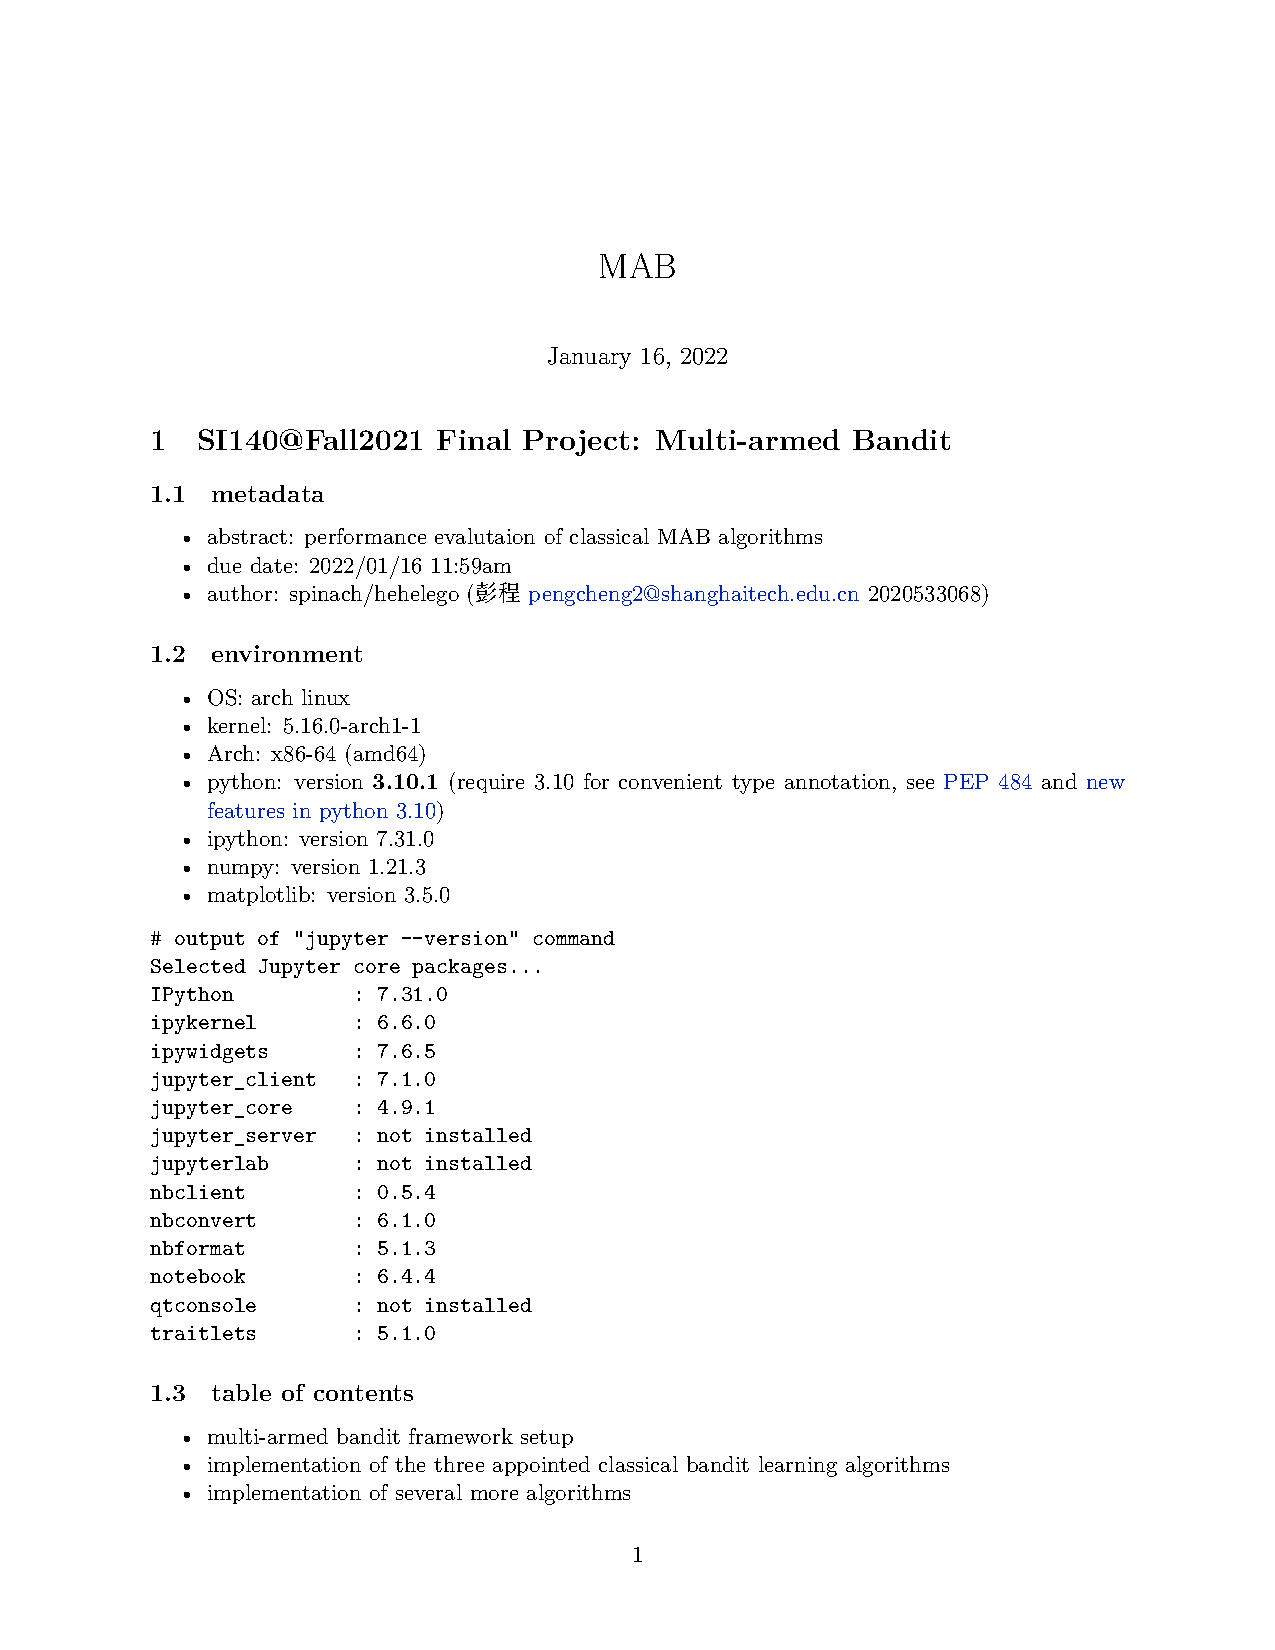
\includepdf[
	pages=-,
	addtotoc={1, section, 1, Python Implementation and Simulation, ipynb}
]{MAB.pdf}
\end{document}
